\documentclass{article}
\usepackage[utf8]{inputenc}


\title{Why ReLU(instead of sigmoid/tanh)?}
\author{}
\date{}

\usepackage{natbib}
\usepackage{graphicx}
\usepackage{amsmath,amssymb}
\usepackage[left=2.5cm,right=2.5cm,top=1cm,bottom=1.25cm]{geometry}
\usepackage{hyperref}
\usepackage{multicol}
\usepackage[export]{adjustbox}
\usepackage{sidecap}
\usepackage{float}
\usepackage[export]{adjustbox}
\hypersetup{colorlinks=true,urlcolor=blue}
\renewcommand{\thesubsection}{\arabic{subsection}.}
\pagenumbering{gobble}
\usepackage{subcaption}


\begin{document}

\maketitle

\section*{ReLU}
The rectified Linear Unit is defined as 
\begin{equation*}
    f(x)=\begin{cases}
    x, & \text{$x \geqslant 0$}.\\
    0, & \text{$x<0$}.
    \end{cases}
\end{equation*}
and its derivative is
\begin{equation*}
    f'(x)=\begin{cases}
    1, & \text{$x\geqslant 0$}.\\
    0, & \text{$x<0$}.
    \end{cases}
\end{equation*}

\section*{Avoiding vanishing gradient}
Lets have a look look at the derivative of the three common activation functions- sigmoid, tanh and relu.
\begin{figure}[H]
    \centering
    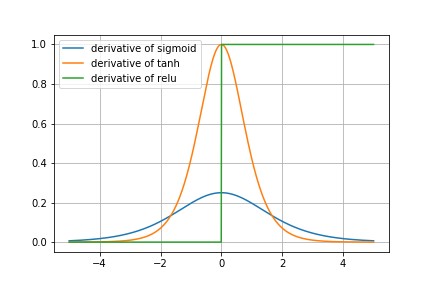
\includegraphics[scale=0.75]{derivatives.png}
    \caption{Residual block}
    \label{fig:Figure 1}
\end{figure}
As evident from the figure derivative of both sigmoid and tanh approaches zero in both direction. What this means is when using gradient descent based algorithm for learning, the propagated error signal becomes smaller and smaller for those those neurons and they hardly contribute to learning at all. This is especially worse when using large number of layers. Because gradient is multiplicative the earlier layers receive less and less gradient even if the error signal is large to begin with. ReLU on the other hand has a derivative one for positive values. So even if the error signal becomes large there is no saturation of gradient and if large number of layers are stacked the propagated error signal does not diminish as it is always multiplied by one. This greatly accelerates the convergence of gradient descent compared to the sigmoid/tanh functions.

\section*{Sparse representations}
The rectified linear activation allows a network to obtain sparse representations(most of the entries are zero). For example, even if we initialize weights with a zero mean normal distribution, around 50\% of the hidden units will have zero valued output. But why should we care about sparse representation? As it turns out neurons in the human brain encode information in sparse and distributed way. Percentage of neurons active at the same time is believed to between 1\% and 4\%. From a computational point of view it provides several benefits. One is we can easily obtain variable size representations. Not all inputs contain same amount of information. We would probably want a lengthy description for high information input compared to the relatively low information inputs. We can just vary the number of active neurons to obtain different length of description. Also sparse representations are more likely to be linearly separable compared to their dense counterpart. It can also reflect original data format. For example in text related tasks where the original data is very sparse. Sparse representations are not highly entangled like the dense ones. Because for dense representation any small variation in the input data will modify most of the entries in the representation vector. But for sparse representation the set of non-zero features will be roughly be the same by small change in the input. In deep learning we want to disentangle the factors explaining the variation in the data.  

\section*{Biological plausibility}
Biological neurons show one sided activation meaning they fire above a certain threshold or not fire at all. ReLU shows this one sided behavior, tanh is anti symmetric around zero which is absent in biological data(sigmoid and tanh are equivalent up to a linear transformation since $tanh(x) = 2\sigma (2x) - 1 $).  

\begin{figure}[H]
  \begin{subfigure}[b]{0.4\textwidth}
    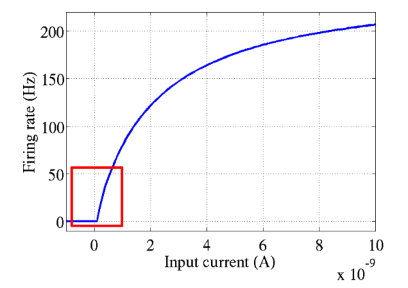
\includegraphics[width=\textwidth]{biological_neuron.png}
    \label{fig:1}
  \end{subfigure}
  \begin{subfigure}[b]{0.45\textwidth}
    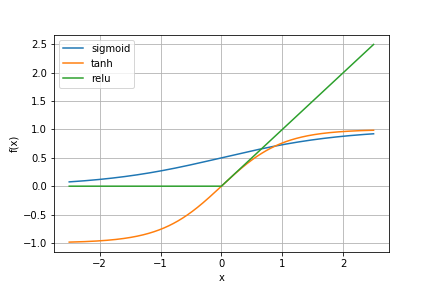
\includegraphics[width=\textwidth]{activations.png}
    \label{fig:2}
  \end{subfigure}
  \caption{\textit{Left:}Common neural activation functions motivated by biological data. \textit{Right:}sigmoid, tanh and relu activation functions}
\end{figure}

\section*{Better gradient direction} The second derivative of ReLU is zero almost everywhere. This means that the gradient direction is far more useful for learning than it would be with activation functions that introduce second-order effects(sigmoid/tanh).

\section*{Computationally cheap}
Computing ReLU and its derivative much cheaper than sigmoid or tanh where one needs to calculate exponential which is costly.

\section*{Potential problems with ReLU}
\begin{itemize}
    \item ReLU is Non-differentiable at zero which might prevent gradient descent based technique to work. However in practice we can just pick a value of 0 or 1 arbitrarily where the input is 0 and it works just fine.
    \item ReLU outputs are not bounded like sigmoid(bounded in $[0, 1]$) or tanh $[-1, +1]$. So when using deeper networks the gradient can blow up the activation. It can be prevented by using techniques like batch normalization or some other forms of regularization.
    \item ReLU neurons can sometimes be pushed into states in which they become inactive for essentially all inputs. In this state, no gradients flow backward through the neuron, and so the neuron becomes stuck in a perpetually inactive state and "dies." This is known as the dying ReLU problem. In some cases, large numbers of neurons in a network can become stuck in dead states, effectively decreasing the model capacity. This problem typically arises when the learning rate is set too high. It may be mitigated by using Leaky ReLUs instead, which assign a small positive slope to the left of x = 0.
    \item Since ReLU doesn't have any form of symmetry, in order to efficiently represent symmetric / antisymmetric behavior in the data, a rectifier network would need twice as many hidden units as a network of symmetric / antisymmetric activation functions like tanh.
\end{itemize}

\section*{Further reading}
\begin{itemize}
    \item \href{http://proceedings.mlr.press/v15/glorot11a/glorot11a.pdf}{Deep Sparse Rectifier Neural Networks}
    \item \href{https://www.iro.umontreal.ca/~lisa/pointeurs/TR1312.pdf}{Learning Deep Architectures for AI}
    \item \href{https://en.wikipedia.org/wiki/Rectifier_(neural_networks)}{Rectifier (neural networks)}
    \item \href{https://arxiv.org/pdf/1502.01852.pdf}{Delving Deep into Rectifiers: Surpassing Human-Level Performance on ImageNet Classification}
\end{itemize}


\end{document}
